\documentclass[twoside]{book}

% Packages required by doxygen
\usepackage{fixltx2e}
\usepackage{calc}
\usepackage{doxygen}
\usepackage[export]{adjustbox} % also loads graphicx
\usepackage{graphicx}
\usepackage[utf8]{inputenc}
\usepackage{makeidx}
\usepackage{multicol}
\usepackage{multirow}
\PassOptionsToPackage{warn}{textcomp}
\usepackage{textcomp}
\usepackage[nointegrals]{wasysym}
\usepackage[table]{xcolor}

% NLS support packages
\usepackage[french]{babel}

% Font selection
\usepackage[T1]{fontenc}
\usepackage[scaled=.90]{helvet}
\usepackage{courier}
\usepackage{amssymb}
\usepackage{sectsty}
\renewcommand{\familydefault}{\sfdefault}
\allsectionsfont{%
  \fontseries{bc}\selectfont%
  \color{darkgray}%
}
\renewcommand{\DoxyLabelFont}{%
  \fontseries{bc}\selectfont%
  \color{darkgray}%
}
\newcommand{\+}{\discretionary{\mbox{\scriptsize$\hookleftarrow$}}{}{}}

% Page & text layout
\usepackage{geometry}
\geometry{%
  a4paper,%
  top=2.5cm,%
  bottom=2.5cm,%
  left=2.5cm,%
  right=2.5cm%
}
\tolerance=750
\hfuzz=15pt
\hbadness=750
\setlength{\emergencystretch}{15pt}
\setlength{\parindent}{0cm}
\setlength{\parskip}{3ex plus 2ex minus 2ex}
\makeatletter
\renewcommand{\paragraph}{%
  \@startsection{paragraph}{4}{0ex}{-1.0ex}{1.0ex}{%
    \normalfont\normalsize\bfseries\SS@parafont%
  }%
}
\renewcommand{\subparagraph}{%
  \@startsection{subparagraph}{5}{0ex}{-1.0ex}{1.0ex}{%
    \normalfont\normalsize\bfseries\SS@subparafont%
  }%
}
\makeatother

% Headers & footers
\usepackage{fancyhdr}
\pagestyle{fancyplain}
\fancyhead[LE]{\fancyplain{}{\bfseries\thepage}}
\fancyhead[CE]{\fancyplain{}{}}
\fancyhead[RE]{\fancyplain{}{\bfseries\leftmark}}
\fancyhead[LO]{\fancyplain{}{\bfseries\rightmark}}
\fancyhead[CO]{\fancyplain{}{}}
\fancyhead[RO]{\fancyplain{}{\bfseries\thepage}}
\fancyfoot[LE]{\fancyplain{}{}}
\fancyfoot[CE]{\fancyplain{}{}}
\fancyfoot[RE]{\fancyplain{}{\bfseries\scriptsize Généré par Doxygen }}
\fancyfoot[LO]{\fancyplain{}{\bfseries\scriptsize Généré par Doxygen }}
\fancyfoot[CO]{\fancyplain{}{}}
\fancyfoot[RO]{\fancyplain{}{}}
\renewcommand{\footrulewidth}{0.4pt}
\renewcommand{\chaptermark}[1]{%
  \markboth{#1}{}%
}
\renewcommand{\sectionmark}[1]{%
  \markright{\thesection\ #1}%
}

% Indices & bibliography
\usepackage{natbib}
\usepackage[titles]{tocloft}
\setcounter{tocdepth}{3}
\setcounter{secnumdepth}{5}
\makeindex

% Hyperlinks (required, but should be loaded last)
\usepackage{ifpdf}
\ifpdf
  \usepackage[pdftex,pagebackref=true]{hyperref}
\else
  \usepackage[ps2pdf,pagebackref=true]{hyperref}
\fi
\hypersetup{%
  colorlinks=true,%
  linkcolor=blue,%
  citecolor=blue,%
  unicode%
}

% Custom commands
\newcommand{\clearemptydoublepage}{%
  \newpage{\pagestyle{empty}\cleardoublepage}%
}

\usepackage{caption}
\captionsetup{labelsep=space,justification=centering,font={bf},singlelinecheck=off,skip=4pt,position=top}

%===== C O N T E N T S =====

\begin{document}

% Titlepage & ToC
\hypersetup{pageanchor=false,
             bookmarksnumbered=true,
             pdfencoding=unicode
            }
\pagenumbering{roman}
\begin{titlepage}
\vspace*{7cm}
\begin{center}%
{\Large E\+S\+P\+R\+IT R\+UN 2000 \\[1ex]\large 1.\+0 }\\
\vspace*{1cm}
{\large Généré par Doxygen 1.8.11}\\
\end{center}
\end{titlepage}
\clearemptydoublepage
\tableofcontents
\clearemptydoublepage
\pagenumbering{arabic}
\hypersetup{pageanchor=true}

%--- Begin generated contents ---
\chapter{Index des structures de données}
\section{Structures de données}
Liste des structures de données avec une brève description \+:\begin{DoxyCompactList}
\item\contentsline{section}{\hyperlink{structBackground}{Background} }{\pageref{structBackground}}{}
\item\contentsline{section}{\hyperlink{structbackground}{background} \\*Struct for background }{\pageref{structbackground}}{}
\item\contentsline{section}{\hyperlink{structPERSONAGE}{P\+E\+R\+S\+O\+N\+A\+GE} \\*Struct for \hyperlink{structPERSONAGE}{P\+E\+R\+S\+O\+N\+A\+GE} }{\pageref{structPERSONAGE}}{}
\item\contentsline{section}{\hyperlink{structvie}{vie} \\*Struct for vie }{\pageref{structvie}}{}
\end{DoxyCompactList}

\chapter{Index des fichiers}
\section{Liste des fichiers}
Liste de tous les fichiers documentés avec une brève description \+:\begin{DoxyCompactList}
\item\contentsline{section}{{\bfseries defs.\+h} }{\pageref{defs_8h}}{}
\item\contentsline{section}{\hyperlink{fonctions_8c}{fonctions.\+c} \\*Testing Program }{\pageref{fonctions_8c}}{}
\item\contentsline{section}{{\bfseries fonctions.\+h} }{\pageref{fonctions_8h}}{}
\item\contentsline{section}{\hyperlink{main_8c}{main.\+c} \\*Testing Program }{\pageref{main_8c}}{}
\end{DoxyCompactList}

\chapter{Documentation des structures de données}
\hypertarget{structBackground}{}\section{Référence de la structure Background}
\label{structBackground}\index{Background@{Background}}
\subsection*{Champs de données}
\begin{DoxyCompactItemize}
\item 
S\+D\+L\+\_\+\+Surface $\ast$ \hyperlink{structBackground_ade7f4649cb1e02ab75167ce898db884c}{background\+Img}
\item 
S\+D\+L\+\_\+\+Surface $\ast$ \hyperlink{structBackground_a4cb0dbd29ce5c40b49b97e5952f84b2f}{background\+Collide}
\item 
S\+D\+L\+\_\+\+Rect \hyperlink{structBackground_a81fdaea521be13c6634186f72b105e33}{background\+Pos}
\end{DoxyCompactItemize}


\subsection{Documentation des champs}
\index{Background@{Background}!background\+Collide@{background\+Collide}}
\index{background\+Collide@{background\+Collide}!Background@{Background}}
\subsubsection[{\texorpdfstring{background\+Collide}{backgroundCollide}}]{\setlength{\rightskip}{0pt plus 5cm}S\+D\+L\+\_\+\+Surface$\ast$ Background\+::background\+Collide}\hypertarget{structBackground_a4cb0dbd29ce5c40b49b97e5952f84b2f}{}\label{structBackground_a4cb0dbd29ce5c40b49b97e5952f84b2f}
Surface \index{Background@{Background}!background\+Img@{background\+Img}}
\index{background\+Img@{background\+Img}!Background@{Background}}
\subsubsection[{\texorpdfstring{background\+Img}{backgroundImg}}]{\setlength{\rightskip}{0pt plus 5cm}S\+D\+L\+\_\+\+Surface$\ast$ Background\+::background\+Img}\hypertarget{structBackground_ade7f4649cb1e02ab75167ce898db884c}{}\label{structBackground_ade7f4649cb1e02ab75167ce898db884c}
Surface \index{Background@{Background}!background\+Pos@{background\+Pos}}
\index{background\+Pos@{background\+Pos}!Background@{Background}}
\subsubsection[{\texorpdfstring{background\+Pos}{backgroundPos}}]{\setlength{\rightskip}{0pt plus 5cm}S\+D\+L\+\_\+\+Rect Background\+::background\+Pos}\hypertarget{structBackground_a81fdaea521be13c6634186f72b105e33}{}\label{structBackground_a81fdaea521be13c6634186f72b105e33}
Rectangle 

La documentation de cette structure a été générée à partir du fichier suivant \+:\begin{DoxyCompactItemize}
\item 
fonctions.\+h\end{DoxyCompactItemize}

\hypertarget{structbackground}{}\section{Référence de la structure background}
\label{structbackground}\index{background@{background}}


struct for background  




{\ttfamily \#include $<$fonctions.\+h$>$}



\subsection{Description détaillée}
struct for background 

La documentation de cette structure a été générée à partir du fichier suivant \+:\begin{DoxyCompactItemize}
\item 
fonctions.\+h\end{DoxyCompactItemize}

\hypertarget{structPERSONAGE}{}\section{Référence de la structure P\+E\+R\+S\+O\+N\+A\+GE}
\label{structPERSONAGE}\index{P\+E\+R\+S\+O\+N\+A\+GE@{P\+E\+R\+S\+O\+N\+A\+GE}}


struct for \hyperlink{structPERSONAGE}{P\+E\+R\+S\+O\+N\+A\+GE}  




{\ttfamily \#include $<$fonctions.\+h$>$}



Graphe de collaboration de P\+E\+R\+S\+O\+N\+A\+GE\+:
\nopagebreak
\begin{figure}[H]
\begin{center}
\leavevmode
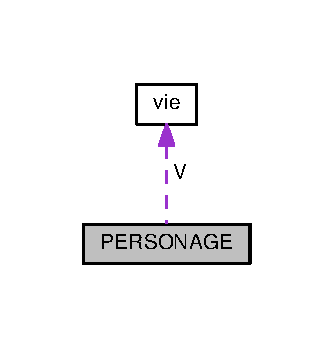
\includegraphics[width=160pt]{structPERSONAGE__coll__graph}
\end{center}
\end{figure}
\subsection*{Champs de données}
\begin{DoxyCompactItemize}
\item 
int \hyperlink{structPERSONAGE_aceab7ab293b56197a8dc153b1aaa2d9e}{score}
\item 
\hyperlink{structvie}{vie} \hyperlink{structPERSONAGE_a55ff47547f25a0a9df67118b91ea58e1}{V}
\item 
char \hyperlink{structPERSONAGE_a6427edb6392463410ad168649b33e410}{nom\+\_\+joueur} \mbox{[}30\mbox{]}
\item 
S\+D\+L\+\_\+\+Rect \hyperlink{structPERSONAGE_a251556a634db6d532af5f928b8a0abe4}{pos\+\_\+perso}
\item 
S\+D\+L\+\_\+\+Surface $\ast$ \hyperlink{structPERSONAGE_a51061ec01fedcce4c8562e043d81cd7a}{tab\+\_\+img} \mbox{[}5\mbox{]}
\item 
S\+D\+L\+\_\+\+Surface $\ast$ \hyperlink{structPERSONAGE_a26a39d344c1ec5d424198c24538f73dc}{surface\+\_\+perso}
\item 
int \hyperlink{structPERSONAGE_a48bc0c626e0210e735c49ba6df5d13e6}{moving}
\item 
int \hyperlink{structPERSONAGE_a1a098d28a8c9867a93df293d4f6731fb}{direction}
\item 
float \hyperlink{structPERSONAGE_aa23d53bb20cc721798d1400f5e121af9}{Mass}
\item 
float \hyperlink{structPERSONAGE_ab3ccb046bb255a27d60b07e2b4df9672}{acceleration}
\item 
float \hyperlink{structPERSONAGE_aaf4734e2f426e60eef271207bc0d3b3d}{velocity}
\end{DoxyCompactItemize}


\subsection{Description détaillée}
struct for \hyperlink{structPERSONAGE}{P\+E\+R\+S\+O\+N\+A\+GE} 

\subsection{Documentation des champs}
\index{P\+E\+R\+S\+O\+N\+A\+GE@{P\+E\+R\+S\+O\+N\+A\+GE}!acceleration@{acceleration}}
\index{acceleration@{acceleration}!P\+E\+R\+S\+O\+N\+A\+GE@{P\+E\+R\+S\+O\+N\+A\+GE}}
\subsubsection[{\texorpdfstring{acceleration}{acceleration}}]{\setlength{\rightskip}{0pt plus 5cm}float P\+E\+R\+S\+O\+N\+A\+G\+E\+::acceleration}\hypertarget{structPERSONAGE_ab3ccb046bb255a27d60b07e2b4df9672}{}\label{structPERSONAGE_ab3ccb046bb255a27d60b07e2b4df9672}
Float \index{P\+E\+R\+S\+O\+N\+A\+GE@{P\+E\+R\+S\+O\+N\+A\+GE}!direction@{direction}}
\index{direction@{direction}!P\+E\+R\+S\+O\+N\+A\+GE@{P\+E\+R\+S\+O\+N\+A\+GE}}
\subsubsection[{\texorpdfstring{direction}{direction}}]{\setlength{\rightskip}{0pt plus 5cm}int P\+E\+R\+S\+O\+N\+A\+G\+E\+::direction}\hypertarget{structPERSONAGE_a1a098d28a8c9867a93df293d4f6731fb}{}\label{structPERSONAGE_a1a098d28a8c9867a93df293d4f6731fb}
Int \index{P\+E\+R\+S\+O\+N\+A\+GE@{P\+E\+R\+S\+O\+N\+A\+GE}!Mass@{Mass}}
\index{Mass@{Mass}!P\+E\+R\+S\+O\+N\+A\+GE@{P\+E\+R\+S\+O\+N\+A\+GE}}
\subsubsection[{\texorpdfstring{Mass}{Mass}}]{\setlength{\rightskip}{0pt plus 5cm}float P\+E\+R\+S\+O\+N\+A\+G\+E\+::\+Mass}\hypertarget{structPERSONAGE_aa23d53bb20cc721798d1400f5e121af9}{}\label{structPERSONAGE_aa23d53bb20cc721798d1400f5e121af9}
Float \index{P\+E\+R\+S\+O\+N\+A\+GE@{P\+E\+R\+S\+O\+N\+A\+GE}!moving@{moving}}
\index{moving@{moving}!P\+E\+R\+S\+O\+N\+A\+GE@{P\+E\+R\+S\+O\+N\+A\+GE}}
\subsubsection[{\texorpdfstring{moving}{moving}}]{\setlength{\rightskip}{0pt plus 5cm}int P\+E\+R\+S\+O\+N\+A\+G\+E\+::moving}\hypertarget{structPERSONAGE_a48bc0c626e0210e735c49ba6df5d13e6}{}\label{structPERSONAGE_a48bc0c626e0210e735c49ba6df5d13e6}
Int \index{P\+E\+R\+S\+O\+N\+A\+GE@{P\+E\+R\+S\+O\+N\+A\+GE}!nom\+\_\+joueur@{nom\+\_\+joueur}}
\index{nom\+\_\+joueur@{nom\+\_\+joueur}!P\+E\+R\+S\+O\+N\+A\+GE@{P\+E\+R\+S\+O\+N\+A\+GE}}
\subsubsection[{\texorpdfstring{nom\+\_\+joueur}{nom_joueur}}]{\setlength{\rightskip}{0pt plus 5cm}char P\+E\+R\+S\+O\+N\+A\+G\+E\+::nom\+\_\+joueur\mbox{[}30\mbox{]}}\hypertarget{structPERSONAGE_a6427edb6392463410ad168649b33e410}{}\label{structPERSONAGE_a6427edb6392463410ad168649b33e410}
Char \index{P\+E\+R\+S\+O\+N\+A\+GE@{P\+E\+R\+S\+O\+N\+A\+GE}!pos\+\_\+perso@{pos\+\_\+perso}}
\index{pos\+\_\+perso@{pos\+\_\+perso}!P\+E\+R\+S\+O\+N\+A\+GE@{P\+E\+R\+S\+O\+N\+A\+GE}}
\subsubsection[{\texorpdfstring{pos\+\_\+perso}{pos_perso}}]{\setlength{\rightskip}{0pt plus 5cm}S\+D\+L\+\_\+\+Rect P\+E\+R\+S\+O\+N\+A\+G\+E\+::pos\+\_\+perso}\hypertarget{structPERSONAGE_a251556a634db6d532af5f928b8a0abe4}{}\label{structPERSONAGE_a251556a634db6d532af5f928b8a0abe4}
Rectangle \index{P\+E\+R\+S\+O\+N\+A\+GE@{P\+E\+R\+S\+O\+N\+A\+GE}!score@{score}}
\index{score@{score}!P\+E\+R\+S\+O\+N\+A\+GE@{P\+E\+R\+S\+O\+N\+A\+GE}}
\subsubsection[{\texorpdfstring{score}{score}}]{\setlength{\rightskip}{0pt plus 5cm}int P\+E\+R\+S\+O\+N\+A\+G\+E\+::score}\hypertarget{structPERSONAGE_aceab7ab293b56197a8dc153b1aaa2d9e}{}\label{structPERSONAGE_aceab7ab293b56197a8dc153b1aaa2d9e}
Int \index{P\+E\+R\+S\+O\+N\+A\+GE@{P\+E\+R\+S\+O\+N\+A\+GE}!surface\+\_\+perso@{surface\+\_\+perso}}
\index{surface\+\_\+perso@{surface\+\_\+perso}!P\+E\+R\+S\+O\+N\+A\+GE@{P\+E\+R\+S\+O\+N\+A\+GE}}
\subsubsection[{\texorpdfstring{surface\+\_\+perso}{surface_perso}}]{\setlength{\rightskip}{0pt plus 5cm}S\+D\+L\+\_\+\+Surface$\ast$ P\+E\+R\+S\+O\+N\+A\+G\+E\+::surface\+\_\+perso}\hypertarget{structPERSONAGE_a26a39d344c1ec5d424198c24538f73dc}{}\label{structPERSONAGE_a26a39d344c1ec5d424198c24538f73dc}
Surface \index{P\+E\+R\+S\+O\+N\+A\+GE@{P\+E\+R\+S\+O\+N\+A\+GE}!tab\+\_\+img@{tab\+\_\+img}}
\index{tab\+\_\+img@{tab\+\_\+img}!P\+E\+R\+S\+O\+N\+A\+GE@{P\+E\+R\+S\+O\+N\+A\+GE}}
\subsubsection[{\texorpdfstring{tab\+\_\+img}{tab_img}}]{\setlength{\rightskip}{0pt plus 5cm}S\+D\+L\+\_\+\+Surface$\ast$ P\+E\+R\+S\+O\+N\+A\+G\+E\+::tab\+\_\+img\mbox{[}5\mbox{]}}\hypertarget{structPERSONAGE_a51061ec01fedcce4c8562e043d81cd7a}{}\label{structPERSONAGE_a51061ec01fedcce4c8562e043d81cd7a}
Surface \index{P\+E\+R\+S\+O\+N\+A\+GE@{P\+E\+R\+S\+O\+N\+A\+GE}!V@{V}}
\index{V@{V}!P\+E\+R\+S\+O\+N\+A\+GE@{P\+E\+R\+S\+O\+N\+A\+GE}}
\subsubsection[{\texorpdfstring{V}{V}}]{\setlength{\rightskip}{0pt plus 5cm}{\bf vie} P\+E\+R\+S\+O\+N\+A\+G\+E\+::V}\hypertarget{structPERSONAGE_a55ff47547f25a0a9df67118b91ea58e1}{}\label{structPERSONAGE_a55ff47547f25a0a9df67118b91ea58e1}
Vie \index{P\+E\+R\+S\+O\+N\+A\+GE@{P\+E\+R\+S\+O\+N\+A\+GE}!velocity@{velocity}}
\index{velocity@{velocity}!P\+E\+R\+S\+O\+N\+A\+GE@{P\+E\+R\+S\+O\+N\+A\+GE}}
\subsubsection[{\texorpdfstring{velocity}{velocity}}]{\setlength{\rightskip}{0pt plus 5cm}float P\+E\+R\+S\+O\+N\+A\+G\+E\+::velocity}\hypertarget{structPERSONAGE_aaf4734e2f426e60eef271207bc0d3b3d}{}\label{structPERSONAGE_aaf4734e2f426e60eef271207bc0d3b3d}
Float 

La documentation de cette structure a été générée à partir du fichier suivant \+:\begin{DoxyCompactItemize}
\item 
fonctions.\+h\end{DoxyCompactItemize}

\hypertarget{structvie}{}\section{Référence de la structure vie}
\label{structvie}\index{vie@{vie}}


struct for vie  




{\ttfamily \#include $<$fonctions.\+h$>$}

\subsection*{Champs de données}
\begin{DoxyCompactItemize}
\item 
S\+D\+L\+\_\+\+Rect \hyperlink{structvie_a2c449c68f658579371dd947f2c801e3d}{pos\+\_\+vie}
\item 
int \hyperlink{structvie_a869d0f8aa7f186ea5117f7e8df5c3be6}{val}
\item 
S\+D\+L\+\_\+\+Surface $\ast$ \hyperlink{structvie_a979731322bbb07c11075b549718f6416}{tab\+\_\+img} \mbox{[}4\mbox{]}
\item 
S\+D\+L\+\_\+\+Surface $\ast$ \hyperlink{structvie_ab10f55c6b06a5ea9d29c38eb44633e37}{surface\+\_\+vie}
\end{DoxyCompactItemize}


\subsection{Description détaillée}
struct for vie 

\subsection{Documentation des champs}
\index{vie@{vie}!pos\+\_\+vie@{pos\+\_\+vie}}
\index{pos\+\_\+vie@{pos\+\_\+vie}!vie@{vie}}
\subsubsection[{\texorpdfstring{pos\+\_\+vie}{pos_vie}}]{\setlength{\rightskip}{0pt plus 5cm}S\+D\+L\+\_\+\+Rect vie\+::pos\+\_\+vie}\hypertarget{structvie_a2c449c68f658579371dd947f2c801e3d}{}\label{structvie_a2c449c68f658579371dd947f2c801e3d}
Rectangle \index{vie@{vie}!surface\+\_\+vie@{surface\+\_\+vie}}
\index{surface\+\_\+vie@{surface\+\_\+vie}!vie@{vie}}
\subsubsection[{\texorpdfstring{surface\+\_\+vie}{surface_vie}}]{\setlength{\rightskip}{0pt plus 5cm}S\+D\+L\+\_\+\+Surface$\ast$ vie\+::surface\+\_\+vie}\hypertarget{structvie_ab10f55c6b06a5ea9d29c38eb44633e37}{}\label{structvie_ab10f55c6b06a5ea9d29c38eb44633e37}
Surface \index{vie@{vie}!tab\+\_\+img@{tab\+\_\+img}}
\index{tab\+\_\+img@{tab\+\_\+img}!vie@{vie}}
\subsubsection[{\texorpdfstring{tab\+\_\+img}{tab_img}}]{\setlength{\rightskip}{0pt plus 5cm}S\+D\+L\+\_\+\+Surface$\ast$ vie\+::tab\+\_\+img\mbox{[}4\mbox{]}}\hypertarget{structvie_a979731322bbb07c11075b549718f6416}{}\label{structvie_a979731322bbb07c11075b549718f6416}
Surface \index{vie@{vie}!val@{val}}
\index{val@{val}!vie@{vie}}
\subsubsection[{\texorpdfstring{val}{val}}]{\setlength{\rightskip}{0pt plus 5cm}int vie\+::val}\hypertarget{structvie_a869d0f8aa7f186ea5117f7e8df5c3be6}{}\label{structvie_a869d0f8aa7f186ea5117f7e8df5c3be6}
Int 

La documentation de cette structure a été générée à partir du fichier suivant \+:\begin{DoxyCompactItemize}
\item 
fonctions.\+h\end{DoxyCompactItemize}

\chapter{Documentation des fichiers}
\hypertarget{fonctions_8c}{}\section{Référence du fichier fonctions.\+c}
\label{fonctions_8c}\index{fonctions.\+c@{fonctions.\+c}}


Testing Program.  


{\ttfamily \#include $<$S\+D\+L/\+S\+D\+L.\+h$>$}\\*
{\ttfamily \#include $<$S\+D\+L/\+S\+D\+L\+\_\+image.\+h$>$}\\*
{\ttfamily \#include $<$stdio.\+h$>$}\\*
{\ttfamily \#include \char`\"{}defs.\+h\char`\"{}}\\*
{\ttfamily \#include \char`\"{}fonctions.\+h\char`\"{}}\\*
Graphe des dépendances par inclusion de fonctions.\+c\+:\nopagebreak
\begin{figure}[H]
\begin{center}
\leavevmode
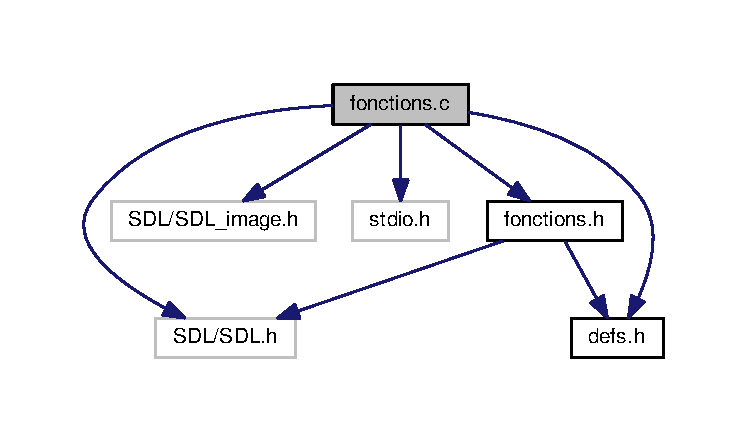
\includegraphics[width=350pt]{fonctions_8c__incl}
\end{center}
\end{figure}
\subsection*{Fonctions}
\begin{DoxyCompactItemize}
\item 
void \hyperlink{fonctions_8c_a2fc4a26bc908975d513c079e2f366aec}{init\+Perso} (\hyperlink{structPERSONAGE}{P\+E\+R\+S\+O\+N\+A\+GE} $\ast$perso)
\begin{DoxyCompactList}\small\item\em to initialise the characters \end{DoxyCompactList}\item 
void \hyperlink{fonctions_8c_a39108d4c6aba3f40f3b16142e074f5a5}{free\+Perso} (\hyperlink{structPERSONAGE}{P\+E\+R\+S\+O\+N\+A\+GE} $\ast$P)
\begin{DoxyCompactList}\small\item\em to frre the characters \end{DoxyCompactList}\item 
int \hyperlink{fonctions_8c_aad1f82eb6e72b4f0b7165f6a10b341a9}{load\+Perso\+Images} (\hyperlink{structPERSONAGE}{P\+E\+R\+S\+O\+N\+A\+GE} $\ast$perso)
\begin{DoxyCompactList}\small\item\em to load the characters pictures \end{DoxyCompactList}\item 
void \hyperlink{fonctions_8c_abf02d44e155c4ce52319ef802acaf98f}{move\+Perso} (\hyperlink{structPERSONAGE}{P\+E\+R\+S\+O\+N\+A\+GE} $\ast$P, \hyperlink{structBackground}{Background} $\ast$B, Uint32 dt)
\begin{DoxyCompactList}\small\item\em to move the characters \end{DoxyCompactList}\item 
int \hyperlink{fonctions_8c_aa8244c3d8654d4cc4a93c96e717bfa04}{load\+Background} (\hyperlink{structBackground}{Background} $\ast$Backg)
\begin{DoxyCompactList}\small\item\em to load the background Backg. \end{DoxyCompactList}\item 
void \hyperlink{fonctions_8c_a87c0db24a7d3d7a15da30c98a14976b4}{init\+Background} (\hyperlink{structBackground}{Background} $\ast$Backg)
\begin{DoxyCompactList}\small\item\em to initialise the background Backg. \end{DoxyCompactList}\item 
void \hyperlink{fonctions_8c_a24afb6b60cad85ed678c9475a412928f}{blit\+Background} (\hyperlink{structBackground}{Background} $\ast$Backg, S\+D\+L\+\_\+\+Surface $\ast$screen)
\begin{DoxyCompactList}\small\item\em to show the background b. \end{DoxyCompactList}\item 
void \hyperlink{fonctions_8c_aa713358cd9ee4f9884b9f804875d5f13}{free\+Background} (\hyperlink{structBackground}{Background} $\ast$Backg)
\begin{DoxyCompactList}\small\item\em to free the background b. \end{DoxyCompactList}\item 
int \hyperlink{fonctions_8c_ad9c436fc5815440f57648231b18e2caf}{jouer} (S\+D\+L\+\_\+\+Surface $\ast$screen)
\begin{DoxyCompactList}\small\item\em to play the game \end{DoxyCompactList}\item 
void \hyperlink{fonctions_8c_aa0d25afd64758716ee7c2f94b0b60ec0}{afficher\+\_\+perso} (\hyperlink{structPERSONAGE}{P\+E\+R\+S\+O\+N\+A\+GE} perso, S\+D\+L\+\_\+\+Surface $\ast$screen)
\begin{DoxyCompactList}\small\item\em to show the characters perso. \end{DoxyCompactList}\end{DoxyCompactItemize}


\subsection{Description détaillée}
Testing Program. 

\begin{DoxyAuthor}{Auteur}
axel 
\end{DoxyAuthor}
\begin{DoxyVersion}{Version}
1.\+0 
\end{DoxyVersion}
\begin{DoxyDate}{Date}
Apr 24, 2019 Testing program related to the characters 
\end{DoxyDate}


\subsection{Documentation des fonctions}
\index{fonctions.\+c@{fonctions.\+c}!afficher\+\_\+perso@{afficher\+\_\+perso}}
\index{afficher\+\_\+perso@{afficher\+\_\+perso}!fonctions.\+c@{fonctions.\+c}}
\subsubsection[{\texorpdfstring{afficher\+\_\+perso(\+P\+E\+R\+S\+O\+N\+A\+G\+E perso, S\+D\+L\+\_\+\+Surface $\ast$screen)}{afficher_perso(PERSONAGE perso, SDL_Surface *screen)}}]{\setlength{\rightskip}{0pt plus 5cm}void afficher\+\_\+perso (
\begin{DoxyParamCaption}
\item[{{\bf P\+E\+R\+S\+O\+N\+A\+GE}}]{perso, }
\item[{S\+D\+L\+\_\+\+Surface $\ast$}]{screen}
\end{DoxyParamCaption}
)}\hypertarget{fonctions_8c_aa0d25afd64758716ee7c2f94b0b60ec0}{}\label{fonctions_8c_aa0d25afd64758716ee7c2f94b0b60ec0}


to show the characters perso. 


\begin{DoxyParams}{Paramètres}
{\em screen} & the screen \\
\hline
{\em $\ast$perso} & the characters \\
\hline
\end{DoxyParams}
\begin{DoxyReturn}{Renvoie}
nothing 
\end{DoxyReturn}
\index{fonctions.\+c@{fonctions.\+c}!blit\+Background@{blit\+Background}}
\index{blit\+Background@{blit\+Background}!fonctions.\+c@{fonctions.\+c}}
\subsubsection[{\texorpdfstring{blit\+Background(\+Background $\ast$\+Backg, S\+D\+L\+\_\+\+Surface $\ast$screen)}{blitBackground(Background *Backg, SDL_Surface *screen)}}]{\setlength{\rightskip}{0pt plus 5cm}void blit\+Background (
\begin{DoxyParamCaption}
\item[{{\bf Background} $\ast$}]{Backg, }
\item[{S\+D\+L\+\_\+\+Surface $\ast$}]{screen}
\end{DoxyParamCaption}
)}\hypertarget{fonctions_8c_a24afb6b60cad85ed678c9475a412928f}{}\label{fonctions_8c_a24afb6b60cad85ed678c9475a412928f}


to show the background b. 


\begin{DoxyParams}{Paramètres}
{\em screen} & the screen \\
\hline
{\em b} & the background \\
\hline
\end{DoxyParams}
\begin{DoxyReturn}{Renvoie}
nothing 
\end{DoxyReturn}
\index{fonctions.\+c@{fonctions.\+c}!free\+Background@{free\+Background}}
\index{free\+Background@{free\+Background}!fonctions.\+c@{fonctions.\+c}}
\subsubsection[{\texorpdfstring{free\+Background(\+Background $\ast$\+Backg)}{freeBackground(Background *Backg)}}]{\setlength{\rightskip}{0pt plus 5cm}void free\+Background (
\begin{DoxyParamCaption}
\item[{{\bf Background} $\ast$}]{Backg}
\end{DoxyParamCaption}
)}\hypertarget{fonctions_8c_aa713358cd9ee4f9884b9f804875d5f13}{}\label{fonctions_8c_aa713358cd9ee4f9884b9f804875d5f13}


to free the background b. 


\begin{DoxyParams}{Paramètres}
{\em b} & the background \\
\hline
\end{DoxyParams}
\begin{DoxyReturn}{Renvoie}
nothing 
\end{DoxyReturn}
\index{fonctions.\+c@{fonctions.\+c}!free\+Perso@{free\+Perso}}
\index{free\+Perso@{free\+Perso}!fonctions.\+c@{fonctions.\+c}}
\subsubsection[{\texorpdfstring{free\+Perso(\+P\+E\+R\+S\+O\+N\+A\+G\+E $\ast$\+P)}{freePerso(PERSONAGE *P)}}]{\setlength{\rightskip}{0pt plus 5cm}void free\+Perso (
\begin{DoxyParamCaption}
\item[{{\bf P\+E\+R\+S\+O\+N\+A\+GE} $\ast$}]{P}
\end{DoxyParamCaption}
)}\hypertarget{fonctions_8c_a39108d4c6aba3f40f3b16142e074f5a5}{}\label{fonctions_8c_a39108d4c6aba3f40f3b16142e074f5a5}


to frre the characters 


\begin{DoxyParams}{Paramètres}
{\em $\ast$p} & the \hyperlink{structPERSONAGE}{P\+E\+R\+S\+O\+N\+A\+GE} \\
\hline
\end{DoxyParams}
\begin{DoxyReturn}{Renvoie}
nothing 
\end{DoxyReturn}
\index{fonctions.\+c@{fonctions.\+c}!init\+Background@{init\+Background}}
\index{init\+Background@{init\+Background}!fonctions.\+c@{fonctions.\+c}}
\subsubsection[{\texorpdfstring{init\+Background(\+Background $\ast$\+Backg)}{initBackground(Background *Backg)}}]{\setlength{\rightskip}{0pt plus 5cm}void init\+Background (
\begin{DoxyParamCaption}
\item[{{\bf Background} $\ast$}]{Backg}
\end{DoxyParamCaption}
)}\hypertarget{fonctions_8c_a87c0db24a7d3d7a15da30c98a14976b4}{}\label{fonctions_8c_a87c0db24a7d3d7a15da30c98a14976b4}


to initialise the background Backg. 


\begin{DoxyParams}{Paramètres}
{\em $\ast$\+Backg} & the background \\
\hline
\end{DoxyParams}
\begin{DoxyReturn}{Renvoie}
nothing 
\end{DoxyReturn}
\index{fonctions.\+c@{fonctions.\+c}!init\+Perso@{init\+Perso}}
\index{init\+Perso@{init\+Perso}!fonctions.\+c@{fonctions.\+c}}
\subsubsection[{\texorpdfstring{init\+Perso(\+P\+E\+R\+S\+O\+N\+A\+G\+E $\ast$perso)}{initPerso(PERSONAGE *perso)}}]{\setlength{\rightskip}{0pt plus 5cm}void init\+Perso (
\begin{DoxyParamCaption}
\item[{{\bf P\+E\+R\+S\+O\+N\+A\+GE} $\ast$}]{perso}
\end{DoxyParamCaption}
)}\hypertarget{fonctions_8c_a2fc4a26bc908975d513c079e2f366aec}{}\label{fonctions_8c_a2fc4a26bc908975d513c079e2f366aec}


to initialise the characters 


\begin{DoxyParams}{Paramètres}
{\em $\ast$perso} & the \hyperlink{structPERSONAGE}{P\+E\+R\+S\+O\+N\+A\+GE} \\
\hline
\end{DoxyParams}
\begin{DoxyReturn}{Renvoie}
nothing 
\end{DoxyReturn}
\index{fonctions.\+c@{fonctions.\+c}!jouer@{jouer}}
\index{jouer@{jouer}!fonctions.\+c@{fonctions.\+c}}
\subsubsection[{\texorpdfstring{jouer(\+S\+D\+L\+\_\+\+Surface $\ast$screen)}{jouer(SDL_Surface *screen)}}]{\setlength{\rightskip}{0pt plus 5cm}int jouer (
\begin{DoxyParamCaption}
\item[{S\+D\+L\+\_\+\+Surface $\ast$}]{screen}
\end{DoxyParamCaption}
)}\hypertarget{fonctions_8c_ad9c436fc5815440f57648231b18e2caf}{}\label{fonctions_8c_ad9c436fc5815440f57648231b18e2caf}


to play the game 


\begin{DoxyParams}{Paramètres}
{\em screen} & the screen \\
\hline
\end{DoxyParams}
\begin{DoxyReturn}{Renvoie}
int 
\end{DoxyReturn}
\index{fonctions.\+c@{fonctions.\+c}!load\+Background@{load\+Background}}
\index{load\+Background@{load\+Background}!fonctions.\+c@{fonctions.\+c}}
\subsubsection[{\texorpdfstring{load\+Background(\+Background $\ast$\+Backg)}{loadBackground(Background *Backg)}}]{\setlength{\rightskip}{0pt plus 5cm}int load\+Background (
\begin{DoxyParamCaption}
\item[{{\bf Background} $\ast$}]{Backg}
\end{DoxyParamCaption}
)}\hypertarget{fonctions_8c_aa8244c3d8654d4cc4a93c96e717bfa04}{}\label{fonctions_8c_aa8244c3d8654d4cc4a93c96e717bfa04}


to load the background Backg. 


\begin{DoxyParams}{Paramètres}
{\em $\ast$\+Backg} & the background \\
\hline
\end{DoxyParams}
\begin{DoxyReturn}{Renvoie}
int 
\end{DoxyReturn}
\index{fonctions.\+c@{fonctions.\+c}!load\+Perso\+Images@{load\+Perso\+Images}}
\index{load\+Perso\+Images@{load\+Perso\+Images}!fonctions.\+c@{fonctions.\+c}}
\subsubsection[{\texorpdfstring{load\+Perso\+Images(\+P\+E\+R\+S\+O\+N\+A\+G\+E $\ast$perso)}{loadPersoImages(PERSONAGE *perso)}}]{\setlength{\rightskip}{0pt plus 5cm}int load\+Perso\+Images (
\begin{DoxyParamCaption}
\item[{{\bf P\+E\+R\+S\+O\+N\+A\+GE} $\ast$}]{perso}
\end{DoxyParamCaption}
)}\hypertarget{fonctions_8c_aad1f82eb6e72b4f0b7165f6a10b341a9}{}\label{fonctions_8c_aad1f82eb6e72b4f0b7165f6a10b341a9}


to load the characters pictures 


\begin{DoxyParams}{Paramètres}
{\em $\ast$perso} & the Personage \\
\hline
\end{DoxyParams}
\begin{DoxyReturn}{Renvoie}
int 
\end{DoxyReturn}
\index{fonctions.\+c@{fonctions.\+c}!move\+Perso@{move\+Perso}}
\index{move\+Perso@{move\+Perso}!fonctions.\+c@{fonctions.\+c}}
\subsubsection[{\texorpdfstring{move\+Perso(\+P\+E\+R\+S\+O\+N\+A\+G\+E $\ast$\+P, Background $\ast$\+B, Uint32 dt)}{movePerso(PERSONAGE *P, Background *B, Uint32 dt)}}]{\setlength{\rightskip}{0pt plus 5cm}void move\+Perso (
\begin{DoxyParamCaption}
\item[{{\bf P\+E\+R\+S\+O\+N\+A\+GE} $\ast$}]{P, }
\item[{{\bf Background} $\ast$}]{B, }
\item[{Uint32}]{dt}
\end{DoxyParamCaption}
)}\hypertarget{fonctions_8c_abf02d44e155c4ce52319ef802acaf98f}{}\label{fonctions_8c_abf02d44e155c4ce52319ef802acaf98f}


to move the characters 


\begin{DoxyParams}{Paramètres}
{\em $\ast$P} & the \hyperlink{structPERSONAGE}{P\+E\+R\+S\+O\+N\+A\+GE} \\
\hline
{\em b} & the background \\
\hline
{\em dt} & the Uint32 \\
\hline
\end{DoxyParams}
\begin{DoxyReturn}{Renvoie}
nothing 
\end{DoxyReturn}

\hypertarget{main_8c}{}\section{Référence du fichier main.\+c}
\label{main_8c}\index{main.\+c@{main.\+c}}


Testing Program.  


{\ttfamily \#include $<$S\+D\+L/\+S\+D\+L\+\_\+image.\+h$>$}\\*
{\ttfamily \#include $<$stdio.\+h$>$}\\*
{\ttfamily \#include $<$stdlib.\+h$>$}\\*
{\ttfamily \#include $<$S\+D\+L/\+S\+D\+L.\+h$>$}\\*
{\ttfamily \#include \char`\"{}defs.\+h\char`\"{}}\\*
{\ttfamily \#include \char`\"{}fonctions.\+h\char`\"{}}\\*
Graphe des dépendances par inclusion de main.\+c\+:
\nopagebreak
\begin{figure}[H]
\begin{center}
\leavevmode
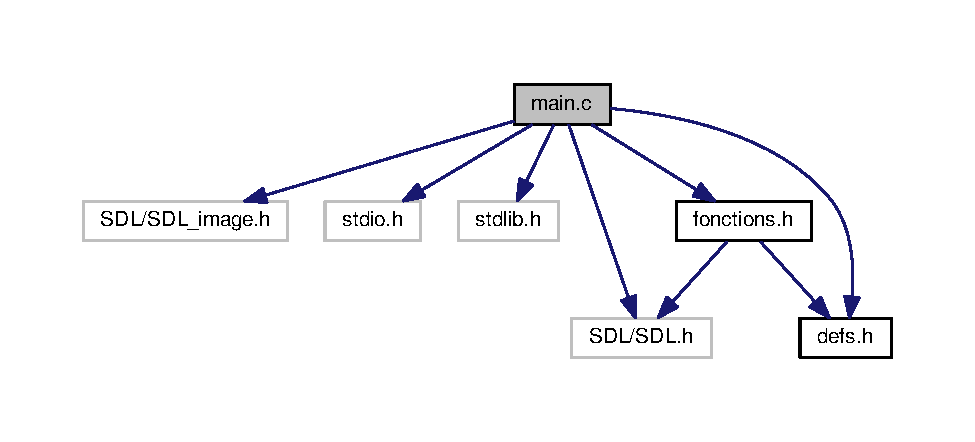
\includegraphics[width=350pt]{main_8c__incl}
\end{center}
\end{figure}
\subsection*{Fonctions}
\begin{DoxyCompactItemize}
\item 
int {\bfseries main} (int argc, char $\ast$$\ast$argv)\hypertarget{main_8c_a3c04138a5bfe5d72780bb7e82a18e627}{}\label{main_8c_a3c04138a5bfe5d72780bb7e82a18e627}

\end{DoxyCompactItemize}


\subsection{Description détaillée}
Testing Program. 

\begin{DoxyAuthor}{Auteur}
axel 
\end{DoxyAuthor}
\begin{DoxyVersion}{Version}
1.\+0 
\end{DoxyVersion}
\begin{DoxyDate}{Date}
Apr 24, 2019 Testing the main 
\end{DoxyDate}

%--- End generated contents ---

% Index
\backmatter
\newpage
\phantomsection
\clearemptydoublepage
\addcontentsline{toc}{chapter}{Index}
\printindex

\end{document}
